\section{Redes SOM}\label{som}
Mapas auto-organizáveis ou Mapas de Kohonen são um tipo de rede neural. Foram desenvolvidos em 1982 por Tuevo
Kohonen, professor emérito da Academia da Finlândia. SelfOrganizing mapas são apropriadamente chamado. "Auto-organização" é porque a supervisão não é
necessária. SOMs aprendem por conta própria através da aprendizagem competitiva não supervisionada.
"Mapas" significa que eles tentam mapear seus pesos para entrar em conformidade com os determinados
dados de entrada. Os nós de uma rede SOM tentam tornar-se igual às entradas 
que lhes são apresentados. Neste sentido, é assim que eles aprendem. Especificamente, o relacionamento topológico das entradas de entrados topológicos
são conservados quando mapeado para uma rede SOM. Isso tem um valor sensato
para a representação de dados complexos.

\subsection{Estrutura}

A Figura \ref{som-node} é uma rede SOM 4x4 (4 nós para baixo, quatro nós de diâmetro). 
cada mapa está ligado a cada nó de entrada. Para este pequeno nó 4x4
de rede, resulta em 4x4x3 = 48 ligações. Em segundo lugar, perceber que nós do mapa não são
ligados uns aos outros. Os nós são organizados desta maneira, como uma grade de duas dimensões
faz com que seja fácil de visualizar os resultados. Esta representação é também útil quando o
Algoritmo SOM é usado. Nesta configuração, cada nó tem um única coordenada (i, j).
Isto torna mais fácil de fazer referência a um nó na rede, e
calcular as distâncias entre os nós. Devido às ligações apenas para o
nós de entrada, os nós mapa são indiferentes quanto ao valor que os seus vizinhos têm.
Um nó de mapa só vai atualizar seus pesos "(explicado a seguir), com base no que o vetor de entrada
fornece de informação.

\begin{figure}[ht]
\centering
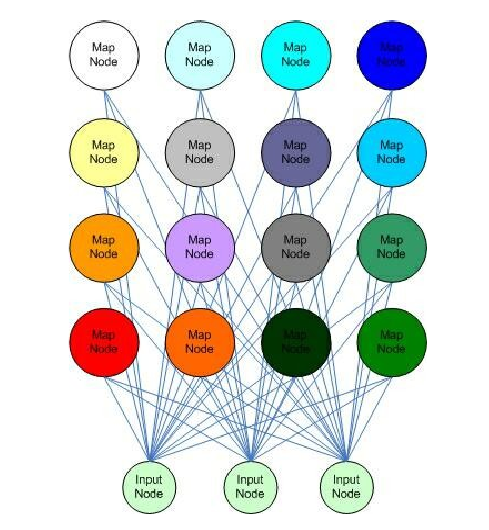
\includegraphics[width=1\textwidth]{imgs/node-som.png}
\caption{Nó do Mapa de Kohonen}
\label{fig:som-node}
\end{figure}